%
%
%

%
% Use the standard article template.
%
\documentclass{article}

% The geometry package allows for easy page formatting.
\usepackage{geometry}
\geometry{letterpaper}

% Load up special logo commands.
\usepackage{doc}

% Package for formatting URLs.
\usepackage{url}

% Packages and definitions for graphics files.
\usepackage{graphicx}
\usepackage{epstopdf}
\DeclareGraphicsRule{.tif}{png}{.png}{`convert #1 `dirname #1`/`basename #1 .tif`.png}

%
% Set the title, author, and date.
%
\title{Predicting Credit Card Defaults}
\author{Jason Brown\\
 M.S. Computer Science \\ Northwestern University \\
  \texttt{jasonbrown2016@u.northwestern.edu}}
\date{March 2016}

%
% The document proper.
%
\begin{document}

% Add the title section.
\maketitle

% Add an abstract.
\abstract{
This paper uses multiple machine learning algorithms, such as K-nearest neighbor, Logistic regression, Discriminant analysis, Naive Bayesian, and Classification tree, to predict credit card defaults from a sample of $n= 30,000$. It uses baseline techniques and seeks to show how selected improvements to the algorithms can be made that result in slightly better model accuracy, as judged by the Receiver Operating Characteristic \textit{area under curve} metric. The paper concludes with a discussion of the strengths and weaknesses of the algorithms, which ones performed the best, and which improvements led to more accurate models.
}

% Add various lists on new pages.
\pagebreak
\tableofcontents

\pagebreak
\listoffigures

\pagebreak
\listoftables

% Start the paper on a new page.
\pagebreak

%
% Body text.
%
\section{Introduction \& Motivation}
\label{introduction}

During the financial crisis that started in 2008, banks did a poor job screening which applicants deserved credit; banks over-lended and creditors over-borrowed. This paper presents how using machine learning techniques can be used to accurately predict which credit card holders are most likely to default; and show how improvements to the baseline methodologies can yield even more accurate predictions.

\section{Problem Description}

\subsection{Description of the Data}

The data is comprised of 23 explanatory variables ($X1$-$X23$) and one response variable ($Y$). The explanatory variables are described in Table~\ref{Explanatory Variables}. $Y$ denotes whether the borrower defaulted on credit card debt repayment, with $Y=1$ denoting default. In the sample size of $n= 30,000$, only $6,636$ ($22\%$) defaulted. \cite{data} \cite{paper}

\begin{table}
\centering
\begin{tabular}{|c|c|c|}\hline
Label & Attribute & Notes \\\hline\hline
X1 & Credit Given &  NT Dollar currency\\
X2 & Gender & 1= male, 2 = female \\
X3 & Education & 1 = grad. school; 2 = university; 3 = high school \\
X4 & Marital Status & 1 = married; 2 = single\\
X5 & Age & years \\
X6 & Repayment Status- Sept & -1 = pay duly; 1 = 1mo payment delay; $\dots$ \\
X7 & Repayment Status- Aug & $\dots$ 9 = 9mo payment delay or greater \\
X8 & Repayment Status- July & -\\
X9 & Repayment Status- June & -\\
X10 & Repayment Status- May & -\\
X11 & Repayment Status- April &- \\
X12 & Bill Statement- Sept & NT Dollary currency \\
X13 & Bill Statement- Aug & -\\
X14 & Bill Statement- July & -\\
X15 & Bill Statement- June &-\\
X16 & Bill Statement- May & -\\
X17 & Bill Statement- April &-\\
X18 & Bill Payment- Sept & NT Dollary currency \\
X19 & Bill Payment- Aug & -\\
X20 & Bill Payment- July & -\\
X21 & Bill Payment- June &-\\
X22 & Bill Payment- May & -\\
X23 & Bill Payment- April &-\\\hline
\end{tabular}

\caption{Explanatory Variables}
\label{Explanatory Variables}
\end{table}

\subsection{Measuring Model Accuracy}

\begin{figure}
\centering
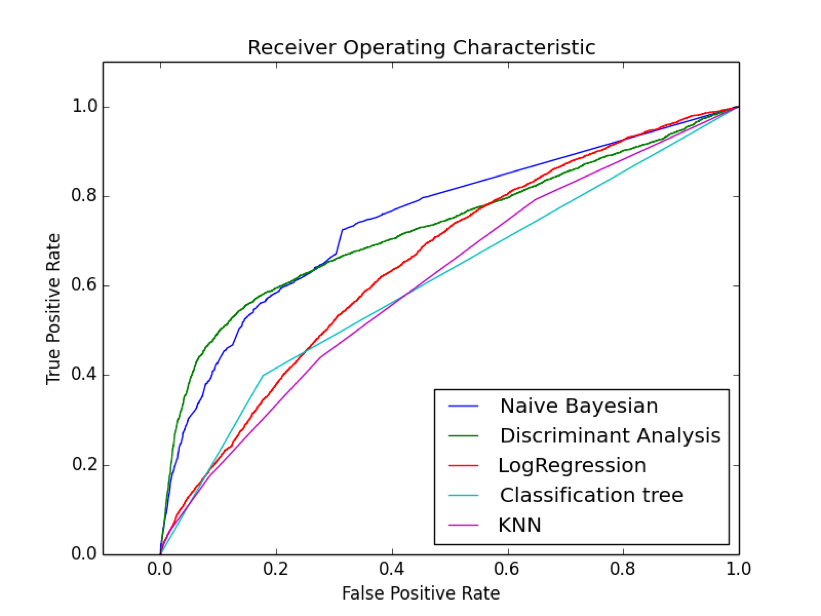
\includegraphics[width=5in]{images/ROC.png} 

\caption{Receiver Operating Characteristic}
\label{ROC area under curve}
\end{figure}

When the explanatory variable is skewed towards one binary value, as is the case here, measuring the accuracy of a model via its error rate is insufficient. Consider a naive model that estimated $\hat{y} = 1$ regardless of the values of the explanatory variables. Despite this being a naive model that added little value, it would have a decent error rate: Consider $n=100$, this model would then have $\approx 22$ misclassifications, resulting in an error rate of 22\%. That's not half-bad!

While error rate is often a good measure of model accuracy, it is clearly insufficient here. A better measure of model accuracy involves using a lift curve. Let's consider a sample of $n=100$ with probability of $y$ of 22\%. Three lines comprise a lift curve: i) the prior probability line which represents a guess; this line would start at (0,0), and extend to (100,22) with slope 11/50. ii) The hypothetical best-model, which would start at (0,0), extend to (22,22) with slope 1, and then extend to (100,22) with slope 0. This curve represents 100\% accuracy, or the ability to pick out which of the 100 samples have response variable equal to one. Lastly, iii) represents the model. This would hopefully be able to ascertain which of the $n=100$ are likely to yield $y=1$, and pick those first. The accuracy measure uses the ratio between the lines ((iii) \& (i)) divided by ((ii) \& (i)). A good model will be closer to the hypothetical best line than to the guess line, so it will have a ratio approaching 1.

Receiver operating characteristic (ROC) \textit{area under curve} is also a good measure of model accuracy. An ROC curve measures the discriminability of a model. It plots the true positive rate as a function of the false positive rate. Each point represents a specificity pair; the curve has higher slope initially because in a gaussian distribution, there are values on both sides of the bell curve that are easy to classify. The slope approaches 0 as the curve gets closer to 100\% true sensitivity rate, as there will always be instances that are very tough to classify, for which the model would yield false positives before it found a true positive. The area under the curve represents the quality of the model, where 1 is the hypothetical best model. The ROC curves for the models utilized in this paper are presented in Figure~\ref{ROC area under curve}. The best performing model had an area under curve ratio of 75\%.

\subsection{Not all Misclassifications are Equal}

\begin{figure}
\centering
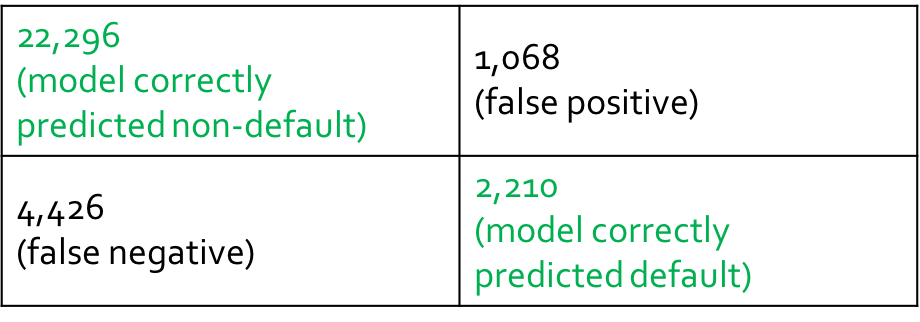
\includegraphics[width=3in]{images/confusion_matrix.png} 

\caption{Confusion Matrix - KNN}
\label{Confusion Matrix - KNN}
\end{figure}

The section above treats a false positive and a false negative equal in the eyes of the model accuracy rates. However, this is not the case in actuality; one misclassification may be considerably more costly to the end user of the model than another type of misclassification. Consider a radiologist screening for cancer; a false positive would scare a patient, but a false negative is far worse - it could lead to the cancer going untreated. Similarly, consider a bank using the credit card data to decide whether to issue credit to a customer. A false positive would represent major loss from default on debt (Figure~\ref{Confusion Matrix - KNN} - upper right quadrant), whereas a false negative would represent a minor loss of revenue from the client under consideration (Figure~\ref{Confusion Matrix - KNN} - lower left quadrant). An interesting area of research would be to determine a good way of dealing with these imbalances in importance of error type.

\section{Baseline Methods}

This section will the discuss the baseline methods used to predict credit card defaults.

\subsection{Classification Tree}

Splitting the data set of $n=30,000$ into $n=15,000$ for training and $n=15,000$ for testing; a decision tree classifier was trained with the training set. A decision tree starts at the root of the tree; each attribute is considered for its \textit{information gain}; whichever attribute best splits the yes / no classifications correctly is chosen as the root of the subtree. \cite{Mitchell} Here, \textit{best} is measured based on relative entropic purity of potential children nodes. Entropy is defined as $$i(N) = - \sum P(w\textsubscript{j}) \cdot \log_{2}{P(w\textsubscript{j})} $$ where $i$ represents the impurity of the node and $P(w\textsubscript{j})$ represents the likelihood of the instance being in class w\textsubscript{j}. An alternative to entropy impurity is gini impurity, whic represents the expected error rate at a given node if the $\hat{y}$ is picked randomly from the prior probabilities of the samples at the given node. \\

A Classification tree (aka Decision tree) model represents a \textit{greedy} algorithm since it is based on making a series of locally-best decisions to build a global optimum. \cite{textbook} This process continues until a base case pure node is reached; in a decision tree, the base case is correct classification; however, pruning can be used in C4.5 and later algorithms to prevent \textit{overfitting} and therefore build a model that generalizes better.\\

Classification tree benefits include:
\begin{itemize}
\item Decision trees can be visualized to help a user further understand the model; this is an advantage over Neural Networks, which are not easily visualized in a way that makes sense to the user.
\item Algorithm is not particularly difficult to implement - easily understood by developer
\item Can handle both numerical and categorical data; a decision boundary at each node is chosen that creates the least impure node. This can be an boolean predicate.
\item Quick to train and efficient to use (a $\hat{y}$ can be produced in $\log_{2}{h}$ where h represents the height of the tree).
\end{itemize}
Classification tree downsides include:
\begin{itemize}
\item Can't represent relatively simple constructs like \&\& or XOR (his was also a drawback of the Perceptron model).
\item Only considers one attribute at a time.
\item Overfitting will occur since the algorithm stops upon reaching a pure node. The can be ameliorated with pruning, or stopping the algorithm sooner based on a threshold improvement in impurity, to help generalize.
\item Minor changes in data can lead to vastly different trees developed during training.
\end{itemize}

\begin{figure}
\centering
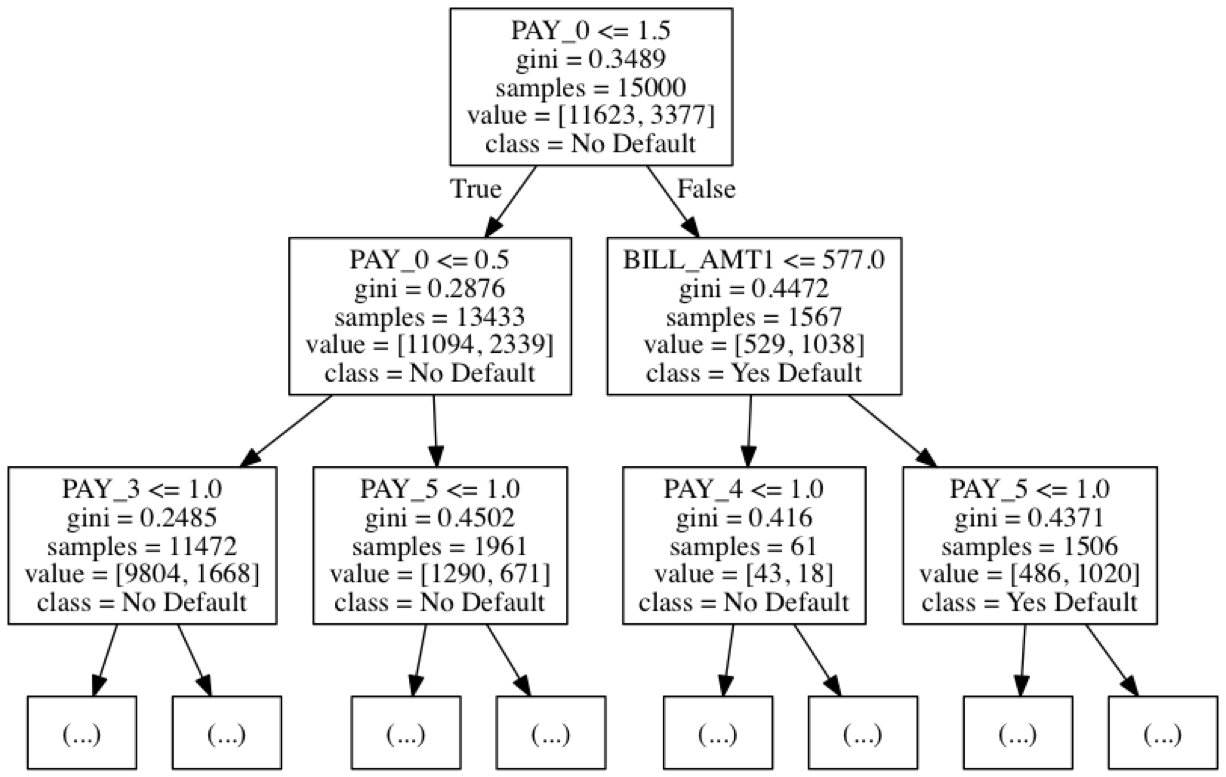
\includegraphics[width=5in]{images/decision_tree_baseline.png} 

\caption{Baseline Decision Tree}
\label{Baseline Decision Tree}
\end{figure}

\subsection{K-Nearest Neighbor}

Using a K-Nearest Neighbor classifier was largely ineffective as a baseline method. It had the lowest ROC area under curve metric at 61\%, and was marginally better than guessing in terms of error rate. \cite{code}\\

K-Nearest Neighbor classifier benefits include:
\begin{itemize}
\item Intuitive; use the closest k neighbors to determine the classification of the instance under consideration
\item Simplicity; a KNN remembers the locations of the elements it's been trained on
\end{itemize}
K-Nearest Neighbor classifier downsides include:
\begin{itemize}
\item Considers all attributes equally, while some may be more correlated to given classification
\item Can be used in supervised and unsupervised environments
\item Unsophisticated; doesn't generate its own model, simply remembers elements trained on
\end{itemize}

\begin{table}
\centering
\begin{tabular}{|c|c|}\hline
K & Error Rate \\\hline\hline
1 & 31\% \\
5 & 25\% \\
10 & 22\% \\
50 & 22\% \\
100 & 22\% \\\hline
\end{tabular}

\caption{KNN k-values and Error Rates; Euclidean distance}
\label{KNN k-values and Error Rates}
\end{table}

\subsection{Logistic Regression}

Logistic regression creates a linear model for classification of K classes via linear functions in $x$. \cite{ML textbook} The sum of the posterior probabilities will sum to 1.  As an example, consider $K=2$; then, this model is just a line that separates the two binary classes. Logistic regression is similar to Classification tree in that a major benefit of it is seeing which attributes are most correlated to the classification. The coefficients tell the user whether the attributes are positively or negatively correlated with the response variable. For the credit card data, the most positive coefficient was X6 at 2.8e-04. The most negative coefficient was X5 at -2.03e-02; these relative values may not mean much because the scales of the data are not equivalently (0,1).

\subsection{Discriminant Analysis}

Discriminant analysis builds a decision surface that is used to separate classes; our analysis was using a linear model that builds a linear decision surface based on the training data. The class prior probabilities can be utilized in the algorithm, though this didn't improve performance. The result of fitting the model is the covariance matrix, coefficients, and y-intercept.

\subsection{Naive Bayesian}

The model is naive in that it presumes independence between features, when this obviously is not correct- for instance, in our data set, being female and having a higher level of education are somewhat correlated (more women graduate from college than men), but the model presumes complete independence. Our model assumed a bernoulli distribution. Naive Bayesian model performed the best in terms of error rate and Receiver operating characteristic area under curve metrics. This is not surprising - it makes sense that each node would contribute some likelihood to the overall likelihood of whether a card holder defaults.

\section{Improvements}

\subsection{Feature Selection}

Visualizing the tree, or viewing an array of the gini importance levels, led to some interesting, but not surprising, information about which attributes were the best predictors of default:
\begin{enumerate}
\item Whether the bill in the prior month was less than 2 months overdue.
\item Whether the bill in the prior month was paid on time.
\item Whether the bill statement amount was less than \$577.
\item Interestingly, demographic information like age, marital status, and education level were much less important attributes.
\end{enumerate}

With only 23 attributes, the goal was not to further reduce the attribute space. While 23! is a decently large space, it is small compared to 500x500 pixel images. When considering the features, the author noticed that \textit{debt ratio} was not included among the 23 attributes. $$debt\_ratio = current\_bill\_statement / total\_credit\_amount $$ This metric was added for the two most recent months, so that the total number of attributes was 25. This had an immediate impact on the decision tree, as shown in Figure~\ref{Decision Tree after Feature augmentation}. Both new ratios, Ratio\_1 and Ratio\_2, were featured near the top of the tree. \\

However, our hypothesis of an improved decision tree was only partially correct. While the new metrics showed up near the top of the tree (indicating relevance), and had decently high gini importance values of 0.03678928 and 0.03428279. their addition to the model did not improve error rates. Prior to the feature selection, the error rate was 18.6\%. Afterwards, it improved to 18.0\%, which is not statistically significant.

\begin{figure}
\centering
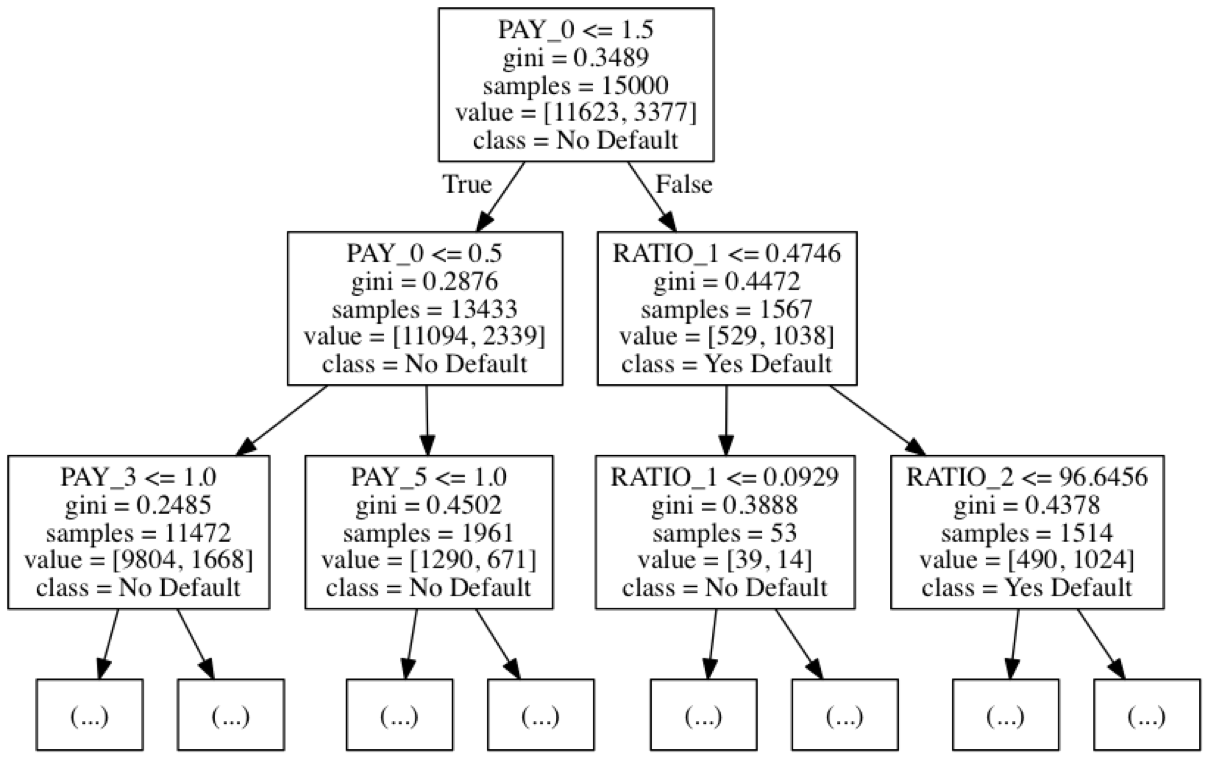
\includegraphics[width=5in]{images/decision_tree_feature_selection.png} 

\caption{Decision Tree after Feature Augmentation; Ratio\_1 and Ratio\_2 added}
\label{Decision Tree after Feature augmentation}
\end{figure}

\begin{table}
\centering
\begin{tabular}{|c|c|c|}\hline
Classifier & 23 - AUC & 25 -AUC \\\hline\hline
Na�ve Bayesian & 74.82\% &  74.71\%\\
Discriminant analysis & 18.2\% &  72.89\%\\
Logistic Regression & 66.58\% &  66.76\%\\
Classification tree & 61.08\% &  61.11\%\\
K-Nearest Neighbor & 61.12\% &  61.12\%\\\hline
\end{tabular}

\caption{Feature Selection Results - 23 versus 25 explanatory variables}
\label{Feature Selection Results}
\end{table}

\subsection{Avoid Overfitting by Mandating Minimum Leaf Size}

The classification tree used to develop a credit card prediction model utilized considered entropic impurity versus Gini impurity. Entropy produced error rates that were $\approx$ 100bp better than Gini impurity. Choosing the minimum number of elements that constituted a leaf node had a major impact on performance. Choosing this to be 40 samples, out of $n= 15,000$, yielded an error rate of 18\%. If it was set as min leaf size of 1, then the error rate was 27\%. That represents a huge difference in testing performance!\\

\subsection{K-fold Cross Validation}

The benefit of K-fold cross validation is that when data is scarce, we can train over more of the data and test on a smaller portion, repeat this process, and average the error rates. This is computationally more demanding and just setting aside a testing set, as the model must be trained K times. When $k=2$, we train over half the data, test over the other half, and then switch and repeat. When $k=n$, we textit{leave one out}, train the model, and test on the one sample left out. This is particularly computationally costly. It results in higher variance since we're only testing on one sample at a time and the models are very similar. In practice, $k=5$ or $k=10$ are reasonable values.  \cite{ML textbook} \\

Our analysis utilized $k=10$. The result was mixed; while it improved the error rate of logistic regression and classification tree methods, it hurt the error rate of discriminant analysis and k-nearest neighbor methods. None were particularly statistically significant. The conclusion may be that with $n=30,000$, using half the data for training and half for testing is reasonable.

\begin{table}
\centering
\begin{tabular}{|c|c|c|c|c|}\hline
Classifier & 50/50 Error Rate & 10-fold Error Rate & 50/50 AUC & 10-fold AUC \\\hline\hline
Na�ve Bayesian & 21.7\% &  21.7\%& 75\% &  74\%\\
Discriminant analysis & 18.2\% &  18.9\%& 73\% &  72\%\\
Logistic Regression & 21.7\% &  22.1\%& 66\% &  65\%\\
Classification tree & 27.3\% &  24.5\%& 61\% &  61\%\\
K-Nearest Neighbor & 24.6\% &  24.5\%& 61\% &  61\%\\
\hline
\end{tabular}

\caption{10-fold cross validation}
\label{10-fold cross validation}
\end{table}

\subsection{Principal Component Analysis}

Principal Component Analysis (PCA) is used to reduce the feature space to a lower dimension, while keeping the most indicative features. The process involves finding the largest eigenvectors of the covariance matrix of the full data; this helps get us the most statistically independent features that still represent the full data. If have have features that are highly correlated with one another, like an image, we may use textit{whitening} to preprocess and reduce redundant data. However, with only 23 credit card attributes, whitening is not necessary. The results of applying PCA on our led to no statistically significant change in model or error rate result.

\begin{table}
\centering
\begin{tabular}{|c|c|c|c|c|}\hline
Classifier & No PCA\_AUC & Apply PCA\_AUC & No PCA\_Error Rate & Apply PCA\_Error Rate \\\hline\hline
Classification tree & 61\% &  54\%& 27.3\% &  34.5\%\\
K-Nearest Neighbor & 61\% &  49\%& 24.6\% &  25.9\%\\
Naive Bayesian & 75\% &  54\%& 21.7\% &  23\%\\
Discriminant analysis & 73\% &  58\%& 18.2\% &  22.5\%\\
Logistic Regression & 66\% &  58\%& 21.7\% &  23.1\%\\
\hline
\end{tabular}

\caption{PCA Results}
\label{PCA Results}
\end{table}

\section{Conclusion}

\begin{table}
\centering
\begin{tabular}{|c|c|c|}\hline
Classifier & Error Rate & ROC\_AUC \\\hline\hline
Na�ve Bayesian & 21.7\% &  75\%\\
Discriminant analysis & 18.2\% &  73\%\\
Logistic Regression & 21.7\% &  66\%\\
Classification tree & 27.3\% &  61\%\\
K-Nearest Neighbor & 24.6\% &  61\%\\\hline
\end{tabular}

\caption{Classifier Performance}
\label{Classifier Performance}
\end{table}

This paper used multiple machine learning algorithms to predict credit card defaults from a sample of $n= 30,000$. It described the pros and cons of each of the baseline techniques, and then showed how the analysis could be improved with improved methodologies. Ultimately, the naive bayesian model performed the best, with an AOC metric of 74\%. This can be explained by each node would contribute some likelihood to the overall likelihood of whether a card holder defaults. The paper considered four improvements: \textit{feature augmentation} impacted the classification tree built in training, but did not improve performance; textit{avoiding model overfitting by mandating minimum leaf size} drastically improved error rates by avoiding overfitting the model; k-fold cross validation had no impact on the data, likely due to the large size of $n$; lastly, PCA did not impact performance either, likely due to the relatively few feature space of X1-X23.\\

While machine learning models were likely in use prior the financial crisis, improvements in the methodologies like the ones described above should help financial institutions build better models as to when a borrower is likely to repay credit card balance; this will help the stability of the borrower, the financial institution, and the economy.



\section{Course Feedback}

Professor Wu is clearly an accomplished researcher and this course is very advanced and well taught; I particularly liked the demos on the chalkboard. Students would have benefited from mandatory assignments from the book to solidify the materials taught in lecture; applying what we've learned helps reenforce learning new material. Similarly, weekly office hours, a teaching assistant, and piazza, would have led to discussions that would have benefited all students and furthered learning. I'm pleased I took the course, and it has opened doors for future statistical pattern recognition learning down-the-road.

\section{Addendum}
All project code available at \url{https://github.com/jb08/credit_card_default_ML}.

\begin{thebibliography} {9}
\bibitem{data} See UC-Irvine Machine Learning Repository, {\sl default of credit card clients }, Jan. 2016
\bibitem{paper} I. Yeh, C. Lien, {\sl The comparisons of data mining techniques for the predictive accuracy of probability of default of credit card clients}, Expert Systems with Applications, 2008
\bibitem{Mitchell}T. Mitchell, {\sl Machine Learning} (McGraw-Hill 1997), chapter 3.
\bibitem{textbook} R. Duda, P. Hart, D. Stork,  {\sl Pattern Classification, 2nd Ed}, 2001.
\bibitem{ML textbook} T. Hastie, R. Tibshirani, J. Friedman {\sl The Elements of Statistical Learning: Data Mining, Inference, and Prediction, 2nd Ed}

\end{thebibliography}

\end{document}
